\documentclass[ % ドキュメントクラス
  uplatex,%upLaTeXを使う
  papersize%紙のサイズがデフォルトと違う場合、PDFにうまく伝える
]{jsarticle}

%% フォント関連
\usepackage{authblk}
\usepackage{diagbox}
\usepackage{bm}
\usepackage[T1]{fontenc} % フォントでT1を使うこと
\usepackage{textcomp} % フォントでTS1を使うこと
\usepackage[utf8]{inputenc} % ファイルがUTF8であること
\usepackage{newpxtext,newpxmath} % ローマンと数式の字体をPalatinoに基づいた新PXフォントで
\usepackage{zi4}%等幅フォントをInconsolataで
\usepackage[multi,deluxe,jis2004]{otf}
\usepackage[prefernoncjk]{pxcjkcat} % なるべく「半角」扱いで。
\cjkcategory{sym18}{cjk} % sym18 (U+25A0 - U+25FF Geometric Shapes) を和文文字あつかい

%% 図表など
% 図の読みこみのために
\usepackage[dvipdfmx, hiresbb]{graphicx, xcolor}
\usepackage{subfigure}
%以下是新增的自定义格式更改
\usepackage[]{caption2} %新增调用的宏包
\renewcommand{\captionlabeldelim}{.~} %重定义分隔符
 %\roman是罗马数字编号,\alph是默认的字母编号,\arabic是阿拉伯数字编号,可按需替换下一行的相应位置
\renewcommand{\thesubfigure}{(\roman{subfigure})}%此外,还可设置图编号显示格式,加括号或者不加括号
\makeatletter \renewcommand{\@thesubfigure}{\thesubfigure \space}%子图编号与名称的间隔设置
\renewcommand{\p@subfigure}{} \makeatother




\usepackage{multirow}
\usepackage{multicol}

\usepackage{booktabs} % 表の横罫線
\usepackage{lscape}  % 表などを90度回転させる

%% 囲み枠
\usepackage{tcolorbox}
\tcbuselibrary{breakable} % ページをまたいで分割できるように

% ソースコードをきれいに出力する
\usepackage{listings}
\lstset{ % 色々な設定
    basicstyle=\ttfamily\tiny, % 基本的にタイプライター体にする
    %numbers=left, % 左側に行番号を表示
    %numberstyle=\small, % 行番号は小さめに
    %numbersep=16pt, % 行番号をどれだけ離すか
    % showspaces=true,% スペースを表示したければtrueにする 
    xleftmargin=15pt, % 左側のマージン
    frame=single, %ソースコードを囲むフレーム
    framesep=10pt, %フレームとコードの間隔
    backgroundcolor=\color[gray]{0.95}, % 背景色
    breaklines=true, % 長い行は改行する
    commentstyle=\color{red},
    keywordstyle=\color{blue}
}
\renewcommand{\lstlistingname}{ソースコード}

% misc
\usepackage{okumacro} % 圏点などのため
\usepackage{pxrubrica} % ルビをつける(okumacroのrubyは使わない)

% hyperrefの設定
\usepackage[dvipdfmx,%
   bookmarks=true,%PDFにしおりをつける
   bookmarksnumbered=true,%しおりに節番号などをつける
   colorlinks=false,%リンクには色をつけない
   hyperfootnotes=false,%脚注からのリンクを作らない
   pdfborder={0 0 0},%枠なし
   pdfpagemode=UseNone]{hyperref}
   

% PDFにしたときの文字化けを防ぐ
\usepackage{pxjahyper}

\title{パターン認識 -- 課題4}

\author{\large GENG Haopeng 611710008 \\ \small Email:  \href{mailto:kevingenghaopeng@gmail.com}{kevingenghaopeng@gmail.com}}

\affil{\small Department of Intelligent Systems, Nagoya University}

\date{\today}

\begin{document}
\maketitle

\begin{abstract}
今回の課題は、多層パーセプトロン、いわばニューラルネットワークによる学習である。課題3での解決しづらい問題、非線形可分離のパターンに応じる分離性能を評価し、irisデータ集を使って学習結果を評価する実験である。
そのほか、課題のソースコードが既に\href{https://github.com/Secondtonumb/pattern_recogn/tree/master/pattern04}{Github Repository}に掲載されるため、解説が備え、参照あるいは実行することは可能である。
\end{abstract}

\section{ニューラルネットワークによる学習(基本編)}
\subsection{実験理論およびアルゴリズム}
この課題は、最急降下法及び誤差逆伝搬法を利用し、ネットワークの各ニューラルの重みやバイオスを修正しつつ、パターンの非線形分離境界を見つける。
学習のアルゴリズム\cite{教科書}は以下のように表す:
\begin{itemize}
\footnotesize
\item[1] 外部から学習パターン、初期重み、バイオを入力する、必要なパラメータ(パターン次元数、クラスター数、ネットワーク層数)を獲得。
\item[2] 初期パラメータを用いてネットワークを築く。
\item[3] 前向き演算: パターン$m$において、
\begin{itemize}
\footnotesize
\item3.1パターン$m$の各次元を入力とする。
\item3.2隠れ層$i$において、ニューラル$j$の入力を計算する。
	$$g_{ij}(\bm{x})=\bm{w_{ij}}^{t}\bm{x_{m}}$$
\item3.3活性化関数を通す。
	$$h_{ij}=S(g_{ij})$$
\item3.4層$i$の出力を層$i+1$の入力とする、step3.2に戻る。
\item3.5全ての層を通過してから、パターン$m$前向き演算終了。
\end{itemize}
\item[4] 後向き演算
\begin{itemize}
\item4.1出力において、全ての学習パターンが収束しているかどうを判断。
\item4.2まだ収束していないパターンのある場合:
\begin{itemize}
\item4.2.1出力層$o$の各ニューラル$j$において、出力$h$を用い、従来の重み$w_{k}$をもたらす誤差$\epsilon$を計算。
	$$\epsilon_{o,j,k}=(h_{o,j}-b{j})h_{o,j}(1-h_{o,j})$$
\item4.2.2隠れ層$i$の各ニューラル$j$において、出力$h$を用い、従来の重み$w_k$をもたらす誤差$\epsilon$を計算。
	$$\epsilon_{i,j,k}=(\sum_{i + 1}\bm{\epsilon_{i+1,\Sigma_{j} } \dot w_{i+1,\Sigma_{j}, i}})h_{i,j,k}(1-h_{i,j,k})$$
\item4.2.3各ニューラルに応じる誤差と従来の重みを用い、重みを修正する。
	$$w_{i,j,k}^{'}=w_{i,j,k}-\epsilon_{i,j,k}h_{i-1,j,k}$$
\end{itemize}
\item4.3全てパターンが収束済みの場合、繰り返し演算終了。
\end{itemize}
\item[5] 学習済みの重みやバイオスを出力。
\end{itemize}
なお、今回の実験条件は表1のように表す。
\begin{table}[h]\footnotesize
\caption{実験条件}
\label{}
\centering
\begin{tabular}{|c|c|c|c|c|c|c|}
\hline
学習パターン数&評価パターン数&パターン次元数&クラスター数&レイヤ数&レイヤごとのニューラル数&重み修正係数\\
\hline
6&1&2&2&2&3&0.1\\
\hline
\end{tabular} 
\end{table}

\subsection{プログラムに工夫した部分}
後ろ向き演算のプロセスは以下のように表す。

\begin{lstlisting}[language=c,caption=Backward Calculation]
     /* Backward */
     
      /* Get Output Layer's Epsilon */
      for(j = 0; j < Clu; j++){
        n_net[Layer - 1][j].e = op_layer_e(label[m][j], n_net[Layer - 1][j].h);
      }
      double e2bcorr[Clu], w2bcorr[Clu];
      /* Get Hidden Layers' Epsilon */
      for(i = Layer - 2; i >= 0; i--){
        for(j = 0; j < Clu; j++){
          e2bcorr[j] = n_net[i + 1][j].e;
        }
        for(j = 0; j < Clu; j++){
          for(k = 0; k < Clu; k++){
            w2bcorr[k] = n_net[i + 1][k].w[j];
          }
          n_net[i][j].e = hid_layer_e(w2bcorr, e2bcorr, n_net[i][j].h);
        }
      }
      /* After Eplison Generated, Update weights */
      /* Layer[1] ~ Layer[<output>] */
      for(i = Layer - 1; i > 0; i--){
        for(j = 0; j < Clu; j++){
          for(k = 0; k < Clu; k++){
            n_net[i][j].w[k] += - rho * n_net[i][j].e * n_net[i - 1][k].h;
          }
          b[i] += - rho * n_net[i][j].e;
        }
      }
      /* Layer[0] */
      for(j = 0; j < Clu; j++){
        for(k = 0; k < Dim; k++){
          n_net[0][j].w[k] += - rho * n_net[0][j].e * init_p[k];
        }
        b[0] += - rho * n_net[0][j].e;
      }
    }
    fprintf(tn_log_file,"\n");
  }
\end{lstlisting}

\subsection{プログラム実行例}
\subsubsection{学習(パラメータ修正)}

各パターンの各クラスターの出力において、訓練プロセスを可視化した。図1は例として、Epochを1000に設定し、各パターンの訓練プロセスである。図1により、パターンに応じるクラスターの出力は最大であり、かつ誤差が小さめの方向に変動している。ゆえに現時点の重みは各学習パターンをうまく分離できることはわかった。

\begin{figure}
\centering
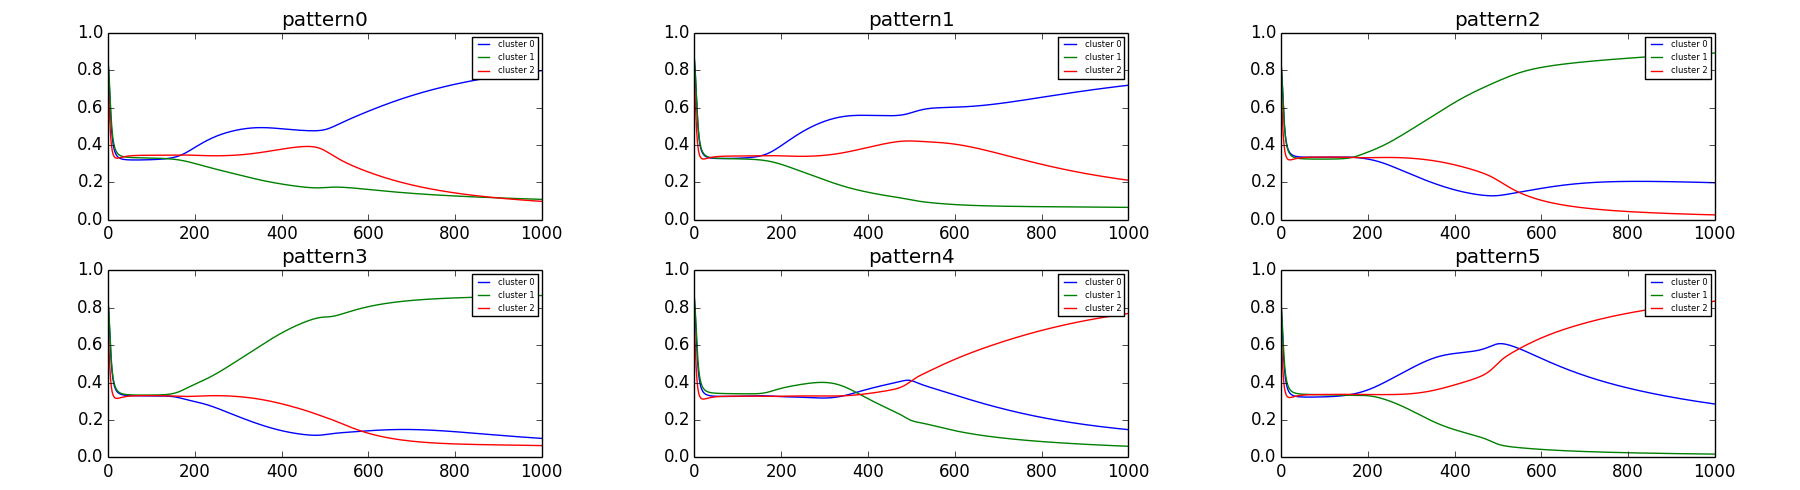
\includegraphics[height=0.25\textwidth]{epoch_1000}
\caption{Training Process(Epoch=1000)} 
\end{figure}

\subsubsection{未知パターン識別}
未知パターン(2, 2)を代入し、出力は以下のようである。ゆえに、Epoch = 1000 の時、正しい識別はできないことがわかった。Epochの設定や収束条件の設定は考察の方に詳しく説明する。
\newpage
\begin{lstlisting}[language=bash,caption=Recognition]
2.000000 2.000000             ---> 各次元
0.942583,0.996466,0.997214,   ---> 出力
Recog result: CLuster[2]      ---> 識別結果
\end{lstlisting}

\subsection{考察}
\subsubsection{収束条件による影響}
より良い学習結果を得るため、収束までの繰り返し演算数(Epoch)をいくつか設定し、分離結果を考察してみた。
収束条件は:
\begin{itemize}
\item[1]弱条件:パターンに応じるクラスターの出力は他のクラスターの出力より大きい場合収束を認める。
\item[2]強条件:パターンに応じるクラスターの出力は上限閾値を超え、かつ他のクラスターの出力は下限閾値以下になる場合収束を認める(ただし、今回は上、下限をそれぞれ0.9、0.1とする)。
\end{itemize}
\begin{figure}[!h]
\centering
\subfigure[epoch=100]{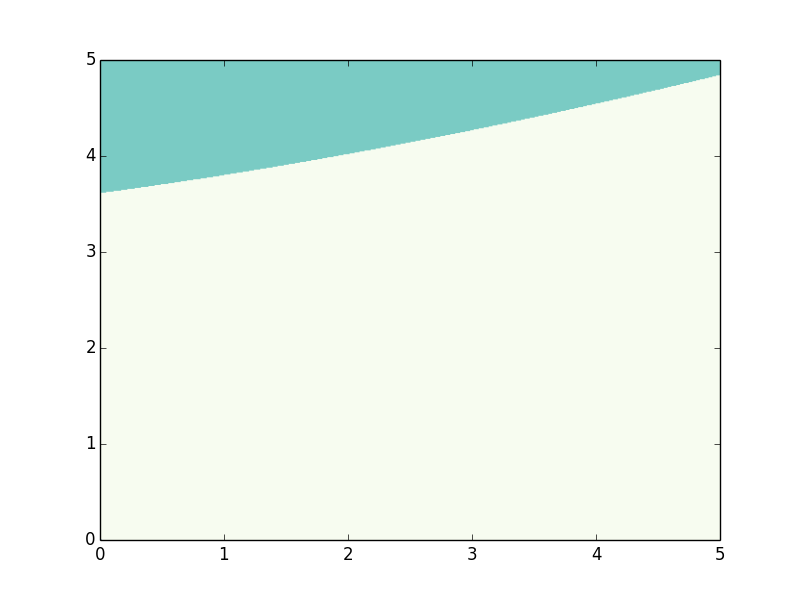
\includegraphics[width=0.25\textwidth] {clu_plots/100}}
\subfigure[epoch = 591(弱条件)]{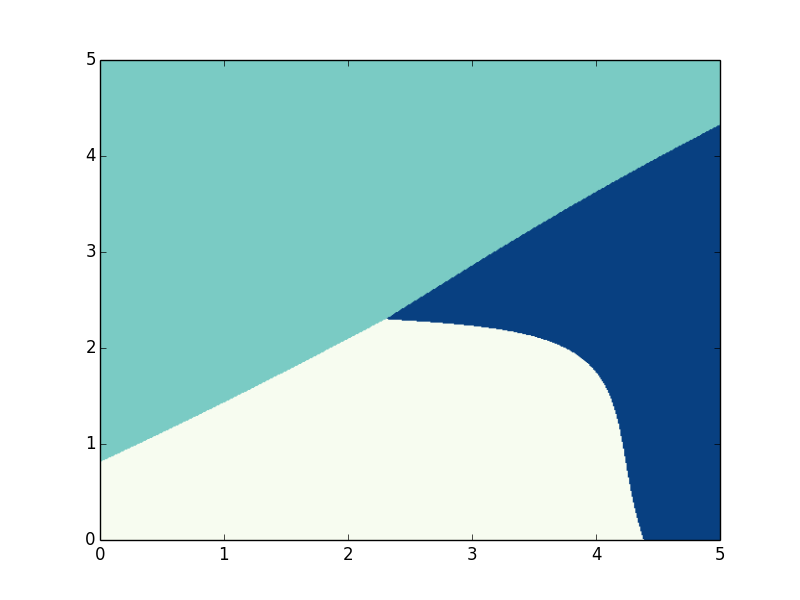
\includegraphics[width=0.25\textwidth] {clu_plots/weak}}
\subfigure[epoch = 1000]{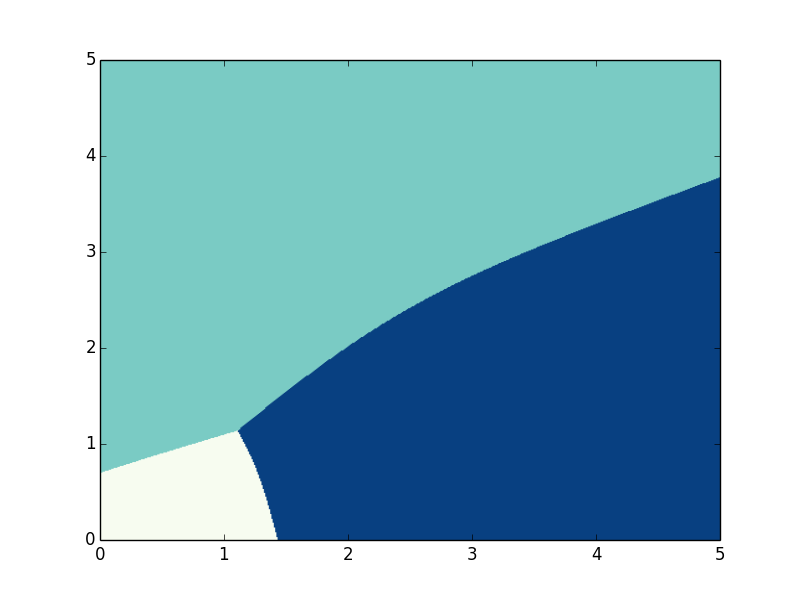
\includegraphics[width=0.25\textwidth] {clu_plots/1000}}
\subfigure[epoch = 1901(強条件)]{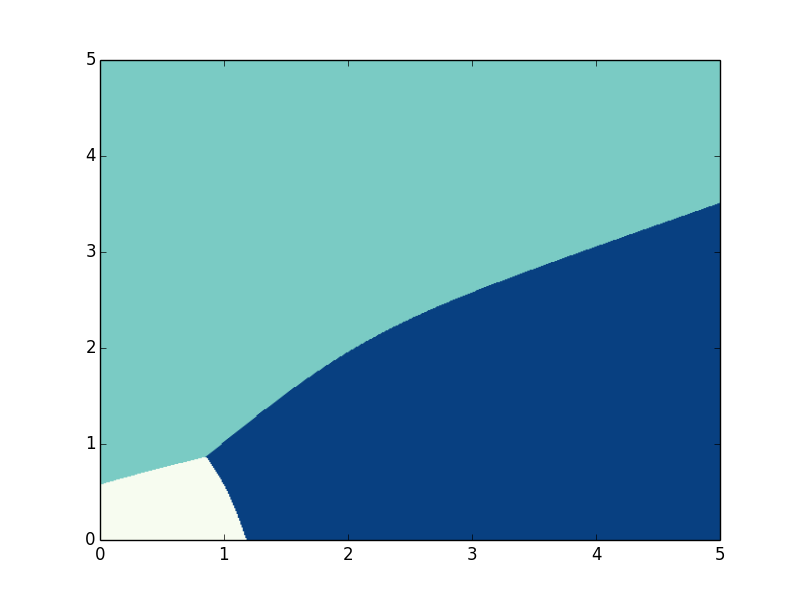
\includegraphics[width=0.25\textwidth] {clu_plots/strong}}
\subfigure[epoch = 10000]{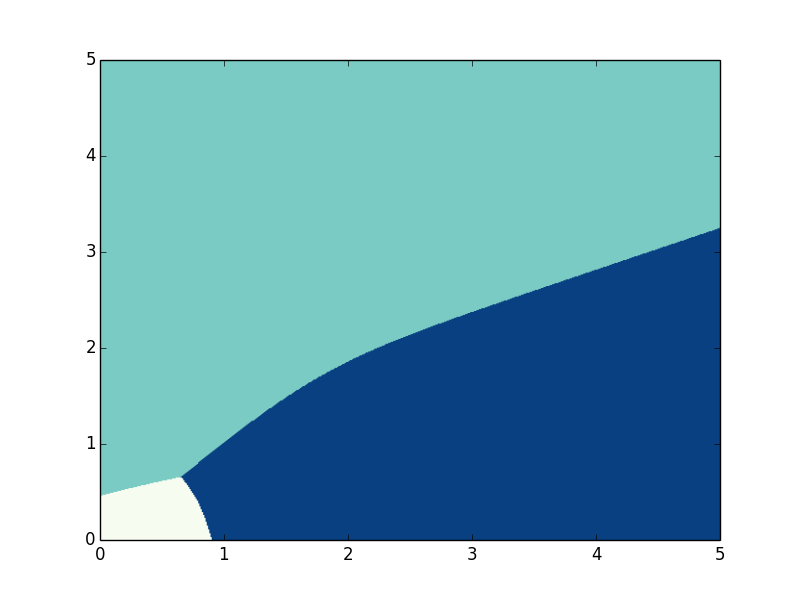
\includegraphics[width=0.25\textwidth] {clu_plots/10000}}
\caption{収束条件による識別境界の変化} 
\end{figure}
図2により、弱条件の場合、ニューラルネットワークの分離状況は理想的であると考えるが、条件が厳しくなると必ずしも識別能力が高くなる、いわば過学習現象\cite{DL}が起こりやすい、ということが判明した。

\section{ニューラルネットワークによる学習(応用編)}
\subsection{実験目的}

上記の実験に基づき、irisデータセット(アヤメの萼片のながさ、幅、花びらのながさ、幅)を学習パターンとし、三種類のアヤメの分離状況を評価し、ニューラルネットワークの学習性能を評価する実験である。ただし、より良い分離性能を得るため、epoch数及びレイヤ数を変数として扱う。
\begin{table}[h]\footnotesize
\caption{iris実験条件}
\label{}
\centering
\begin{tabular}{|c|c|c|c|c|c|c|}
\hline
学習パターン数&評価パターン数&パターン次元数&クラスター数&レイヤごとのニューラル数&重み修正係数\\
\hline
140&10&4&3&3&0.1\\
\hline
\end{tabular} 
\end{table}
\subsection{プログラム実行例}
以下は例としてレイヤ数を2で、収束条件は「弱条件」に設定する時の実行結果である。
\begin{lstlisting}[language=bash,caption=Iris Recognition(2 Layers、Weak Convergence Condition)]
Step2: Training
#         Choose Convergence Condition           #
# [ 0 ] --------  Weak Convergence Condition     #
# [ 1 ] --------  Strong Convergence Condition   #
# [ 2 ] --------  Test Mode(Define Epoch Number) #
0
#    Use Weak Convergence Condition   #
#          Generate Condition         #
#   Output[cluster] > Output[Others]  #

Epoch : 94
Step3: Recognition
Pattern[0]
0.998769,0.917666,0.386239,
True Cluster: [0]	Recog result: [0]
========
Pattern[1]
0.998789,0.916082,0.385725,
True Cluster: [0]	Recog result: [0]
========
Pattern[2]
0.293875,0.985167,0.984565,
True Cluster: [1]	Recog result: [1]
========
Pattern[3]
0.024372,0.910811,0.999029,
True Cluster: [1]	Recog result: [2]
========
Pattern[4]
0.534288,0.992362,0.959099,
True Cluster: [1]	Recog result: [1]
========
Pattern[5]
0.258434,0.983354,0.987012,
True Cluster: [1]	Recog result: [2]
========
Pattern[6]
0.021083,0.902353,0.999162,
True Cluster: [2]	Recog result: [2]
========
Pattern[7]
0.020714,0.901271,0.999177,
True Cluster: [2]	Recog result: [2]
========
Pattern[8]
0.031864,0.924838,0.998724,
True Cluster: [2]	Recog result: [2]
========
Pattern[9]
0.020646,0.901089,0.999179,
True Cluster: [2]	Recog result: [2]
========
Error Rate : 0.200000
\end{lstlisting}
結果により、この時の誤識別率は20.0\%であることが判明した。
\subsection{考察}
レイヤ数と収束条件を実験変量として、考察した結果は表3のように表す。
\begin{table}[h]\footnotesize
\caption{iris実験結果}
\label{}
\centering
\begin{tabular}{|c|c|c|c|c|c|c|}
\hline
\diagbox{レイヤ数}{誤識別率}{収束条件} &epoch=100&epoch=500&epoch=1000&epoch=5000&弱条件&強条件\\
\hline
2&10\%&10\%&10\%&10\%&20\%(epoch=94)&60\%(epoch=25709)\\ 
\hline
3&10\%&50\%&60\%&60\%&20\%(epoch=115)&60\%(epoch=10622)\\ 
\hline
4&80\%&70\%&70\%&60\%&40\%(epoch=205)&60\%(epoch=12430)\\ 
\hline
\end{tabular} 
\end{table}

よって、今回の実験において、レイヤ数とも関わらず、epochが弱条件に近い方の識別率が高い。なお、予想と違って、ネットワークが複雑になればなるほど、識別結果が悪くなる。その原因の一つは、パターンの複雑度(次元数、クラスター数、データ量)がそれほど多くないため、あえて学習能力の高い識別マシンを使うと、識別マシンの容量(capacity)は現在の学習パターンにとって不適切であることと考える。\cite{DL}

そして、実験中他の発見において、初期重みの設定は収束速度と収束結果にかなり影響を与えている。なお、学習パターンの入力順序は実験結果にも影響があることも気づいた。今回においては、ランダムに入力するよりも、一連同じ種類パターンを順序で入力した方(バッチ処理と相似)の実験結果が良いということがわかった。

\section{ニューラルネットワークで遊ぶ}
\href{https://playground.tensorflow.org/}{A Neural Network Playground}で考察した結果は以下のようである。

\begin{itemize}
\footnotesize
\item{1}活性化関数によって、分離性能も異なる。提供された非線形可分離のデータにおいて、$Tanh$の性能は高い。
\item{2}各層のニューラル数は必ずしも多いほうが良い。
\item{3}一部分の学習プロセスにおいて、コスト関数の値は一時的に安定し、さらに不安定になる場合もある。上記の実験の学習プロセスには、似たような現象も起こり得るが。原因はいまいちわからないが、勾配の最急降下法に関する問題であると考える。
\end{itemize}

\begin{figure}[!h]
\centering
\subfigure[Tensorflow]{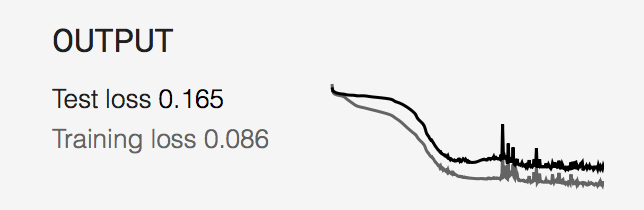
\includegraphics[width=0.4\textwidth] {unstable}}
\subfigure[irisデータ集]{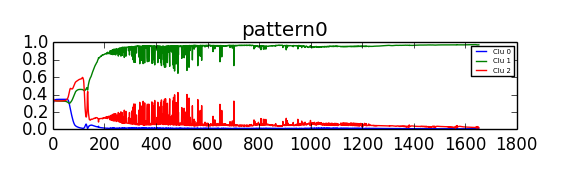
\includegraphics[width=0.4\textwidth] {unstable_test}}
\caption{学習中の不安定現象} 
\end{figure}



\begin{thebibliography}{9}
    \bibitem{教科書} 石井健一郎, 上田修功, 村瀬洋, 等. わかりやすいパターン認識[M]. Ohmsha, 1998.
    \bibitem{DL} Ian Goodfellow,Yoshua Bengio, Aaron Courville. Deep Learning. MIT Press, 2016.
\end{thebibliography}

\end{document}